

\section{RESULTS AND VALIDATION}
The final result of the system being developed is a desktop environment where user can interact with the system through voice command to accomplish the task. The current system consists of simple GUI in the desktop environment that greets user with the greeting message at the welcome screen and then prompts the user to choose one of the available service options using his voice command which in our case is done by using the Nepali Numeral words. Based on the voice command i.e. the number spoken by user typical service is chosen and the response system selects the service option with the number being assigned to it.

The result thus obtained is being analyzed in context of several parameters of the system during various development phases.Result of several phases have been studied and analyzed as discussed below using appropriate constraints of the measurement that are depicted below
in detail.

\subsection{Result}

\subsubsection{Data Sample}
For our project we used Nepali numeral words recognition in order to embed with the interactive response system. Thus for the training of the system training data sets were required. Due to unavailability of data samples we collected the samples from different individuals through a recording software. The details regarding the data samples are tabulated in a table given below:


\begin{center}
	\begin {table}[h]
	\begin{center}
		
	\begin{tabular}{ |c|c| } 
		\hline
		Total number of Samples & 100 Samples per word  \\ 
		\hline
		Recorded Sample Frequency & 16000 Hz  \\ 
		\hline
		Number of Speakers & 20  \\ 
		\hline
	\end{tabular}
\caption{Test data sample details}
\end{center}
\end{table}
\end{center}


\subsubsection{Noise Reduction}

We used Spectral Subtraction method to reduce the additive noise from the speech signal. Based on testing the various level of threshold, we we able to remove the additive noise from the signal and have a mostly clean signal.


Below image shows a noisy signal and the clean noise reduced signal.

\begin{figure}[H]
	\begin{center}
		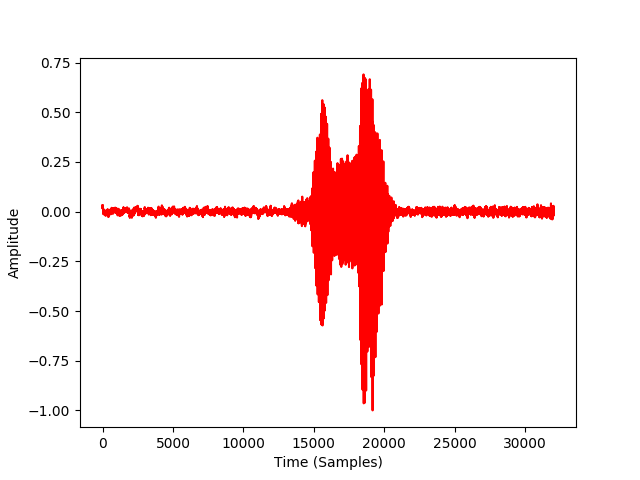
\includegraphics[scale=0.8]{images/mainSigOriginal.png}
		\caption{Original Sound Signal}
		\label{original sound}
	\end{center}
\end{figure}

\begin{figure}[H]
	\begin{center}
		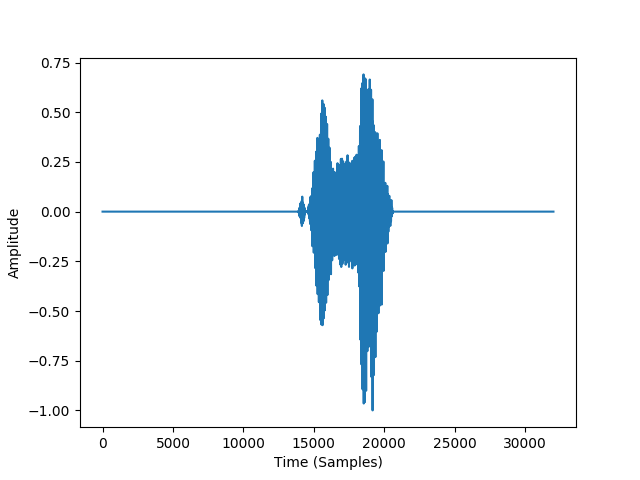
\includegraphics[scale=0.8]{images/mainSigRefine.png}
		\caption{Refined Sound Signal}
		\label{refined sound}
	\end{center}
\end{figure}



The spectrogram below shows the spectral subtraction of average noise.
\begin{figure}[H]
	\begin{center}
		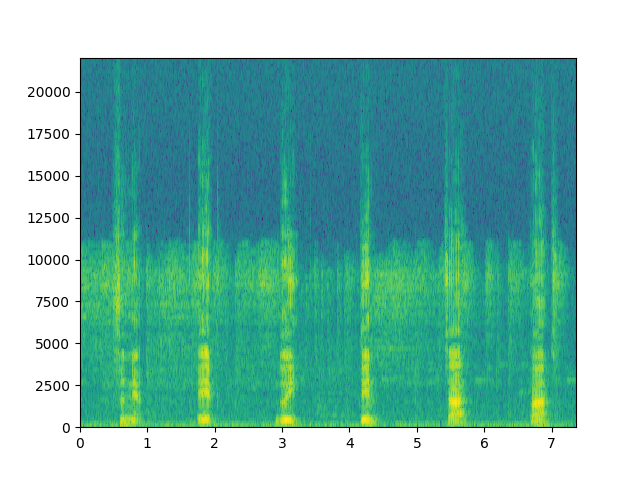
\includegraphics[scale=0.5]{images/main_Spectogram_Original.png}
		\caption{Spectogram of Original Sound Signal}
		\label{Spectro_original}
	\end{center}
\end{figure}

\begin{figure}[h]
	\begin{center}
		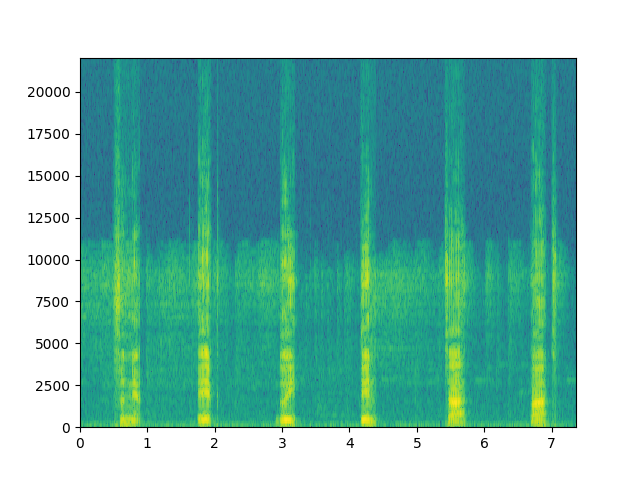
\includegraphics[scale=0.7]{images/MainSpectogram_Refine.png}
		\caption{Spectogram of Refined Sound Signal}
		\label{Spectro_refined}
	\end{center}
\end{figure}


\subsubsection{Silence Removal Module}
	
	During the training sample generation and actual testing, we trimmed away the silence part and extracted only the voiced region. By breaking the sample into chunks and based on the threshold level, we extracted only the voiced sound. 
	
	Below shows the original image and another only the voiced image with trimmed initial and ending silences.
	
	\begin{figure}[H]
		\begin{center}
			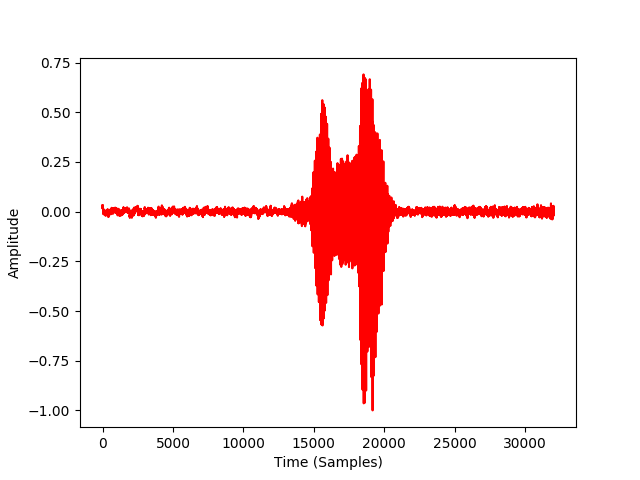
\includegraphics[scale=0.8]{images/mainSigOriginal.png}
			\caption{Original input sound signal}
			\label{orginal}
		\end{center}
	\end{figure}
	
	
	\begin{figure}[H]
		\begin{center}
			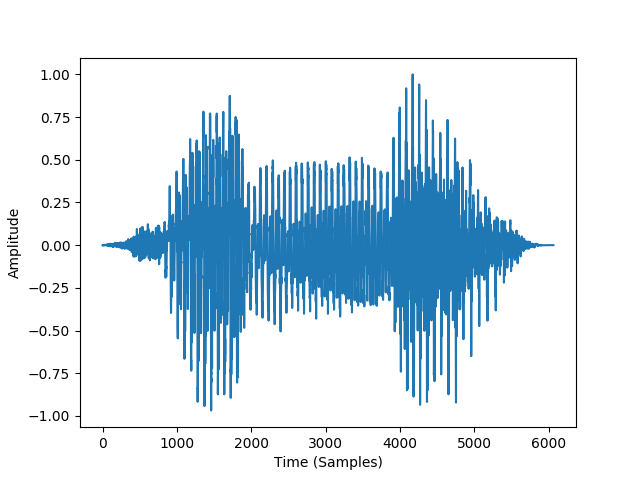
\includegraphics[scale=0.8]{images/voiced_sound.png}
			\caption{Voiced sound signal}
			\label{Voiced}
		\end{center}
	\end{figure}
	
	
	

\subsubsection{HMM Module}


The Output for any speech signal in an HMM module is the probability that the speech signal belongs to that model. We have created different HMM model for each word and the speech signal is passed through every model to predict what are its probability of being in that model. The probability calculated in the Log Probability.

\begin{figure}[H]
	\begin{center}
		
		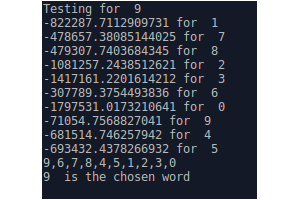
\includegraphics[scale = 1.0]{results_hmm}
		\caption{Log probability result for each model for a speech sample Nepali word 9}
	\end{center}
\end{figure}




\subsubsection{RNN Module}


Recurrent Neural Network can be applied in place of Hidden Markov Model. The output is the number that it predicts after it runs through the sequence of data.

\begin{figure}[H]
	\begin{center}
		
		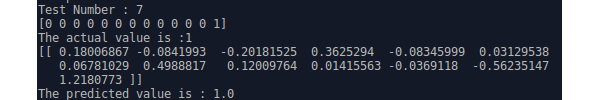
\includegraphics[scale = 0.5]{results_rnn}
		\caption{The result for a word speech of 1 in a RNN module}
	\end{center}
\end{figure}



\subsubsection{Output of the System}

The Result of the overall project is an Interactive Voice Response System. The IVR system is implemented as a desktop application where the user is given a list of options and he can navigate through the options using his speech as input. The system is an overall integration
of Noise Reduction Module, Silence Removal Module, Feature Extraction Module and a prediction module for which either HMM Module or RNN Module can be used.

\begin{figure}[H]
	\begin{center}
		
		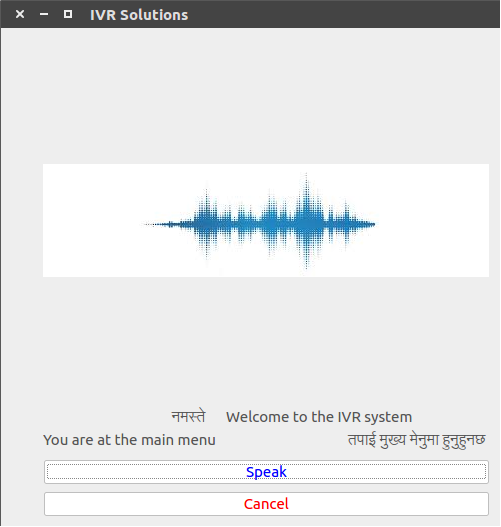
\includegraphics[scale = 0.4]{mainpage}
		\caption{The first GUI interface of the system}
	\end{center}
\end{figure}

\begin{figure}[H]
	\begin{center}
		
		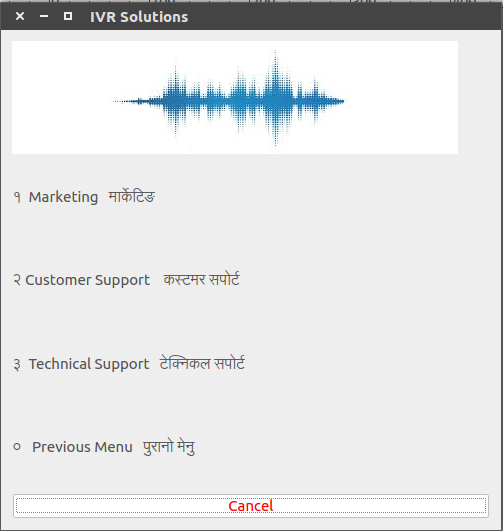
\includegraphics[scale = 0.4]{secondpage}
		\caption{The interface where voice input can be provided to make a selection}
	\end{center}
\end{figure}

\begin{figure}[H]
	\begin{center}
		
		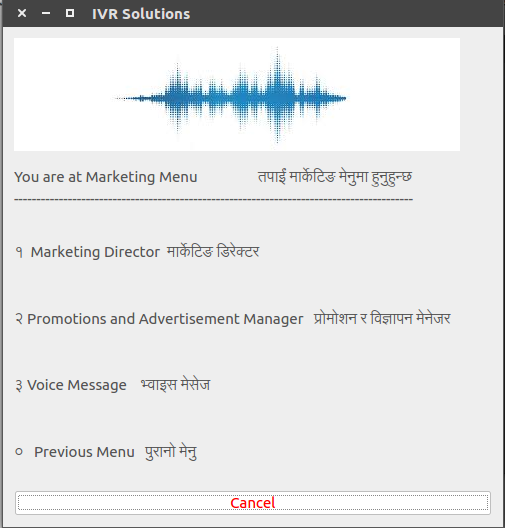
\includegraphics[scale = 0.4]{thirdpage}
		\caption{The interface after the selection has been made where there are again list of options}
	\end{center}
\end{figure}


\subsection{Validation}

The system was validated by checking the number of times it makes the correct prediction for the samples given. The system is an overall integration of Noise Reduction Module, Silence Removal Module, Feature Extraction Module and a prediction module for which either HMM Module or RNN Module can be used. For the initial phase HMM module was chosen as the prediction module.

The approach taken for validation was dividing the samples that we had into training samples and test samples to check how many correct predictions does the sample makes. We used one sample from each word as test data and were able to get an accuracy of around 70 percentage.

\begin{figure}[H]
	\begin{center}
		
		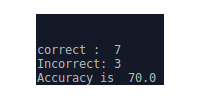
\includegraphics[scale = 1.0]{hmm_accuracy}
		\caption{Accuracy for Test Samples using HMM Module for Prediction}
	\end{center}
\end{figure}

Now the next approach applied for validating the HMM result was by using the live user data to be feed into the HMM. The accuracy was calculated by calculating the total times the HMM model makes correct predictions out of total number of data feed in. In this approach the total accuracy was around 76 percentage.
We can now validate the use of noise reduction module and Silence Removal module using the same system as above . For both Noise Reduction Module and Silence Removal Module, a same approach was take, the system was ran once with the modules in them and once without them and the accuracy were compared.

\begin{center}
	\begin {table}[h]
	\begin{center}
		
		\begin{tabular}{ |c|c| } 
			\hline
			\textbf{Without Noise Reduction Module} & \textbf{With Noise Reduction Module}  \\ 
			\hline
			60.12\% & 74.28\%  \\ 
			\hline
		
		\end{tabular}
		\caption{Accuracy Comparison for Use of Noise Reduction Module}
	\end{center}
\end{table}
\end{center}


\begin{center}
	\begin {table}[h]
	\begin{center}
		
		\begin{tabular}{ |c|c| } 
			\hline
			\textbf{Without Silence Removal Module} & \textbf{With Silence Removal Module}  \\ 
			\hline
			52.12\% & 74.28\%  \\ 
			\hline
			
		\end{tabular}
		\caption{Accuracy Comparison for use of Silence Removal Module}
	\end{center}
\end{table}
\end{center}

Now, we can run similar kind of test while using the RNN prediction module. RNN can be used instead of HMM to use it as a prediction module. We need to first select among the various RNN implementations available. We have got Simple RNN, LSTM RNN and GRU RNN. A test for all these three was run. The test was done by making each module to predict for the same 35 input speech samples.

\begin{figure}[H]
	\begin{center}
		
		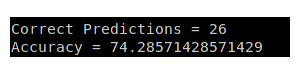
\includegraphics[scale = 0.5]{simple_result}
		\caption{The accuracy while using Simple RNN}
	\end{center}
\end{figure}
\begin{figure}[H]
	\begin{center}
		
		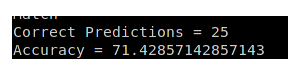
\includegraphics[scale = 0.5]{lstm_result}
		\caption{The accuracy while using LSTM RNN}
	\end{center}
\end{figure}

\begin{figure}[H]
	\begin{center}
		
		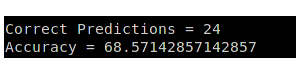
\includegraphics[scale = 0.5]{gru_result}
		\caption{The accuracy while using GRU RNN}
	\end{center}
\end{figure}

\begin{center}
	\begin {table}[h]
	\begin{center}
		
		\begin{tabular}{ |c|c| } 
			\hline
			\textbf{RNN Module} & \textbf{Accuracy}  \\ 
			\hline
			Simple RNN & 74.28\%  \\ 
			\hline
			LSTM & 71.43\%  \\ 
			\hline
			GRU & 68.57\%  \\ 
			\hline			
		\end{tabular}
		\caption{Accuracy Comparison for Various Variations of RNN}
	\end{center}
\end{table}
\end{center}

Now test were run to identify the perfect number of hidden units in the layers. The test was carried out by using various numbers of hidden units to find the optimal one.

\begin{figure}[H]
	\begin{center}
		
		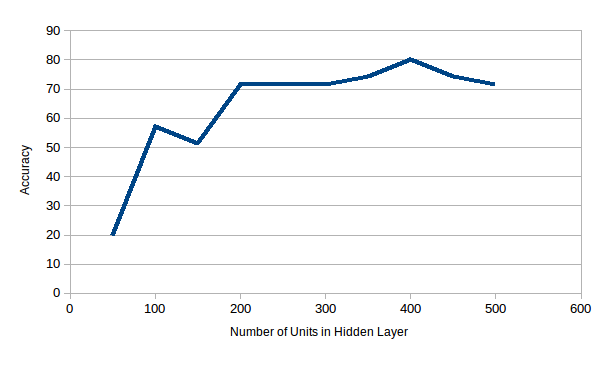
\includegraphics[width = \linewidth]{comparison_rnn}
		\caption{Accuracy for Various number of Hidden Units}
	\end{center}
\end{figure}

The Accuracy calculated till now were based on data samples collected, the sound sample set were distributed in sets of training samples and test samples. Now, the models were tested using real live input audio. The input were given by ten different people each speaking the same number ten times giving each number a live test of 100 samples.

\begin{center}
	\begin {table}[h]
	\begin{center}
		
		\begin{tabular}{ |c|c| } 
			\hline
			Total Number Of Speakers & 10  \\ 
			\hline
			Test given for a Number by each speaker & 10 times \\ 
			\hline
			Total Live Test for a Number & 100  \\ 
			\hline
		\end{tabular}
		\caption{Test Model for Live Data}
	\end{center}
\end{table}
\end{center}

Then the test was carried out and the result obtained can be tabulated as

\begin{center}
	\begin {table}[h]
	\begin{center}
		
		\begin{tabular}{ |c|c|c|c| } 
			\hline
			Word Spoked & Total Times spoken & Correct Prediction(HMM) & Correct Prediction(RNN)    \\ 
			\hline
			Nepali Zero & 100 & 57 & 74  \\
			\hline
			Nepali One & 100 & 62 & 78 \\
			\hline
			Nepali Two & 100 & 65 & 75  \\
			\hline
			Nepali Three & 100 & 63 & 82  \\
			\hline
			Nepali Four & 100 & 69 & 77  \\
			\hline
			Nepali Five & 100 & 55 & 69 \\
			\hline
			Nepali Six & 100 & 72 & 82 \\
			\hline
			Nepali Seven & 100 & 68 & 77 \\ 
			\hline
			Nepali Eight & 100 & 71 & 83  \\
			\hline
			Nepali Nine & 100 & 73 &  78 \\
			\hline
			\textbf{Total} & \textbf{1000} & \textbf{655} &  \textbf{775} \\
			\hline
			
		\end{tabular}
		\caption{Result for Test Carried out on live Data}
	\end{center}
\end{table}
\end{center}

From the above table, the results for live data were also similar as to the previous one. While using HMM, we got accuracy of around 65.5\% and for RNN of around 77.5\% . 



\subsection{Analysis}

From Above results, we can see that the use of Noise Reduction Module and Silence Detection Module gave good accuracy when they were used as compared to when they were not used and are so an integral part of the system. The accuracy of HMM module is good given the fact that we had such a small dataset available and same is the case with RNN module being used.

We got that Simple RNN has better accuracy then GRU and LSTM. Though LSTM and GRU are advancements of Simple RNN, the accuracy of RNN was still high due to the fact that our model is a simple kind of RNN models with not much dependencies so Simple RNN performed better. The Number of hidden units with 400 gave the best result and thus the same one was used for further processing. The best accuracy of 80 percentage while
using simple RNN and 400 hidden cell units was obtained. The accuracy of RNN is better compared to HMM.

The best accuracy that we could obtain was only of 80 percentage. Though this accuracy is less compared to above 95 perecentage accuracy obtained by Google, Baidu, Etc, but our accuracy can be considered fairly good based on the fact that we had a limited number os samples. The accuracy of our system will increase if we can generate more samples.